\documentclass{article}
\usepackage[francais]{babel}
\usepackage[UTF8]{inputenc}
\usepackage[T1]{fontenc}
\usepackage{graphicx}
\usepackage{fancyhdr}
\usepackage{eurosym}
\usepackage{color}
\usepackage{soul}

\pagestyle{fancyplain} \chead{}\lhead{\textit{Les Professionnels}} \rhead{\emph{\textit{Evasion}}}

\definecolor{pseudorouge}{RGB}{200, 50, 50}
\definecolor{pseudoblue}{RGB}{20,10,230}

\begin{document}
\thispagestyle{empty}
\begin{center}
\fontsize{21}{21}{\textbf{Rapport de Soutenance 2 \vspace*{0.2cm}\newline\textit{Evasion}}}
\end{center}

\vspace*{0.7cm}

\begin{center}
\fontsize{21}{21}{\textbf{- Les Professionnels/}}
\fontsize{21}{21}{\textbf{2013-2014 -}}
\end{center}

\vspace*{0.5cm}

\begin{center}

\includegraphics[scale=01.0]{evasion}
\end{center}

\vspace*{0.5cm}

\fontsize{14}{14}
\begin{center}
{Lenny \textcolor{pseudorouge}{\textit{"Le Noob"}} Danino - danino\_l}
\end{center}
\begin{center}
Louis \textcolor{pseudoblue}{\textit{"El Parain"}} Kédémos - kedemo\_l
\end{center}
\begin{center}
Anatole \textcolor{pseudoblue}{\textit{"Totonut"}} Moreau - moreau\_a
\end{center}
\begin{center}
Khalis Chalabi - chalab\_k
\end{center}

\begin{center}

\includegraphics[scale=00.20]{infini}
\end{center}

\newpage
\thispagestyle{empty}
\tableofcontents

\newpage
\fontsize{12}{12}
\pagenumbering{arabic}
\section{Introduction}
\par
Plus de deux mois se sont écoulés depuis la 1ère soutenance et on peut dire qu’on a bien progressé !
Durant cette période nous avons d’abord pris un laps de temps de repos mais qui permis de mieux nous reconcentrer pour la suite.
De ce fait nous avons terminé une partie des taches qui nous incombées de faire pour cette soutenance depuis la première et puisque nous aimons déjà notre jeu nous avons fait en sorte de le rendre vraiment beau !
\newline
\par
Par rapport à nos prévisions il va de soi qu’elles ont été respectées malgré nos épreuves importantes qui ont marqué nos emplois du temps.
Actuellement notre jeu est déjà à un stade intéressant puisque dorénavant on peut avoir un bon aperçu des décors, des personnages, du multijoueur…
\newline
\par
Aujourd’hui notre groupe est plus que soudé, tant par le temps que nous avons passé ensemble  que par  l'importance que nous éprouvons tous pour ce projet. Cela s’est fait en partageant nos désirs, problèmes rencontrés et idées. Plusieurs fois nous avons décidé de se retrouver pour parler et programmer ensemble, de manière plus efficace. 
\newline
\par
Notre précédente note nous a encouragés à donner le meilleur de nous-mêmes, pour avoir une identique et même plus ! Ce projet est donc devenu un véritable engouement pour chacun et c’est toujours avec plaisir que nous nous retrouvons, à la différence d’un simple groupe qui n’accorderais aucune ou peu d’importance à ce projet.
\newline
\par
Nous avons écouté les remarques faites lors de la première soutenance et avons tout fait pour que cette fois, le jeu vous plaise encore plus. Notre site a été refait et certains d’entre nous se sont concentrés davantage sur le code pour rendre le jeu réellement fonctionnel.
\newline
\par
Malgré cela, la soutenance n'en reste pas moins un certain défi, que nous espérons relever pour continuer sur notre lancée.
Ce rapport détaillera donc les nouvelles caractéristiques du jeu et présentera également les prévisions pour la soutenance suivante.

\newpage

\section{Avancements}
\subsection{Louis\textcolor{pseudoblue}{\textit{"El Parrain"}} Kedemos}

\subsubsection{Expérience personnelle}
\newpage

\subsection{Khalis Chalabi}

\subsubsection{Avancement du projet}

\newpage

\subsection{Lenny \textcolor{red}{"Le Noob"} Danino}
\subsubsection{Personnages/Décors}

\par
Les textures des personnages sont des éléments très important dans le jeu car elles sont ce qui est immédiatement regardé par les joueurs. Il faut qu’elles soient jolies et agréables sinon les joueurs ne voudront pas jouer au jeu. Ainsi nous avons décidé qu’il serait préférable de dessiner par-dessus des textures provenant d’images sur internet. Cela apporte un degré de réalisme non négligeable.
\newline
\newline
\underline{Réalisations:}

\par
\underline{Les textures et le code:}
\newline

\par
Premièrement il a fallu réaliser un modèle de base pour les personnages découpé avec Blender.  Ce logiciel est extrêmement utile mais je n’y avais jamais touché et il m’a donc fallu l’aide de Louis et de tutos pour parvenir à me débrouiller suffisamment. Nous avons préféré rendre notre personnage cubique. C’était intéressant à faire car cela nécessitait de visualiser l’ensemble dans l’espace comme lorsqu’on découpe un cube.
\begin{center}
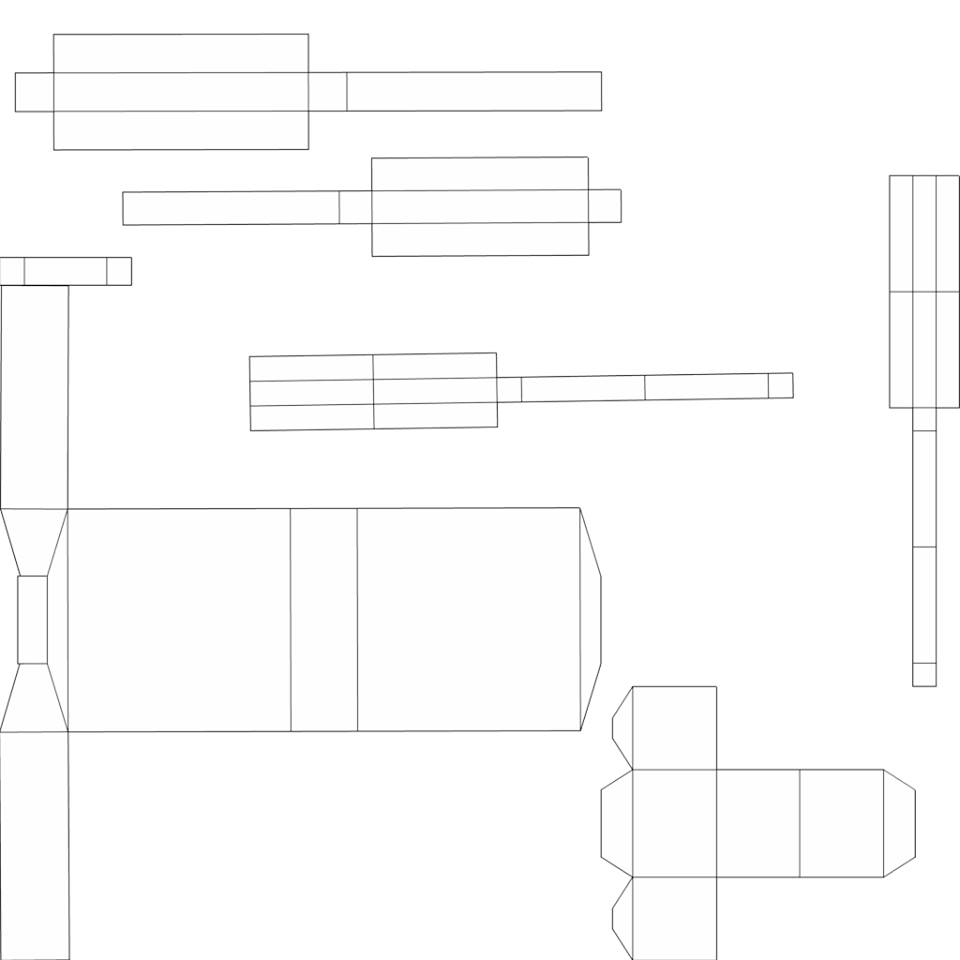
\includegraphics[scale=0.3]{decoupe.jpg}
\end{center}
\newpage
En me basant sur le modèle j’ai pu créer les textures de 2 personnages. J’ai utilisé Photoshop, qui comme Blender m’était entièrement inconnu, pour la correction des images et la découpe. Puis j’ai visualisé le résultat avec Blender. Je vous présente donc le Pnj des prisonniers :
\newline

\begin{center}
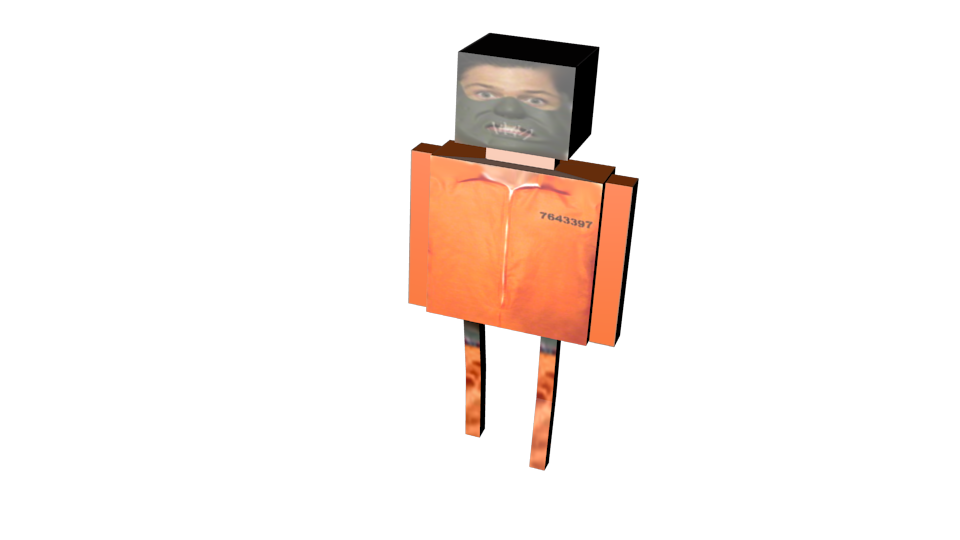
\includegraphics[scale=0.8]{prisonnierblend.png}
\end{center}
\begin{center}
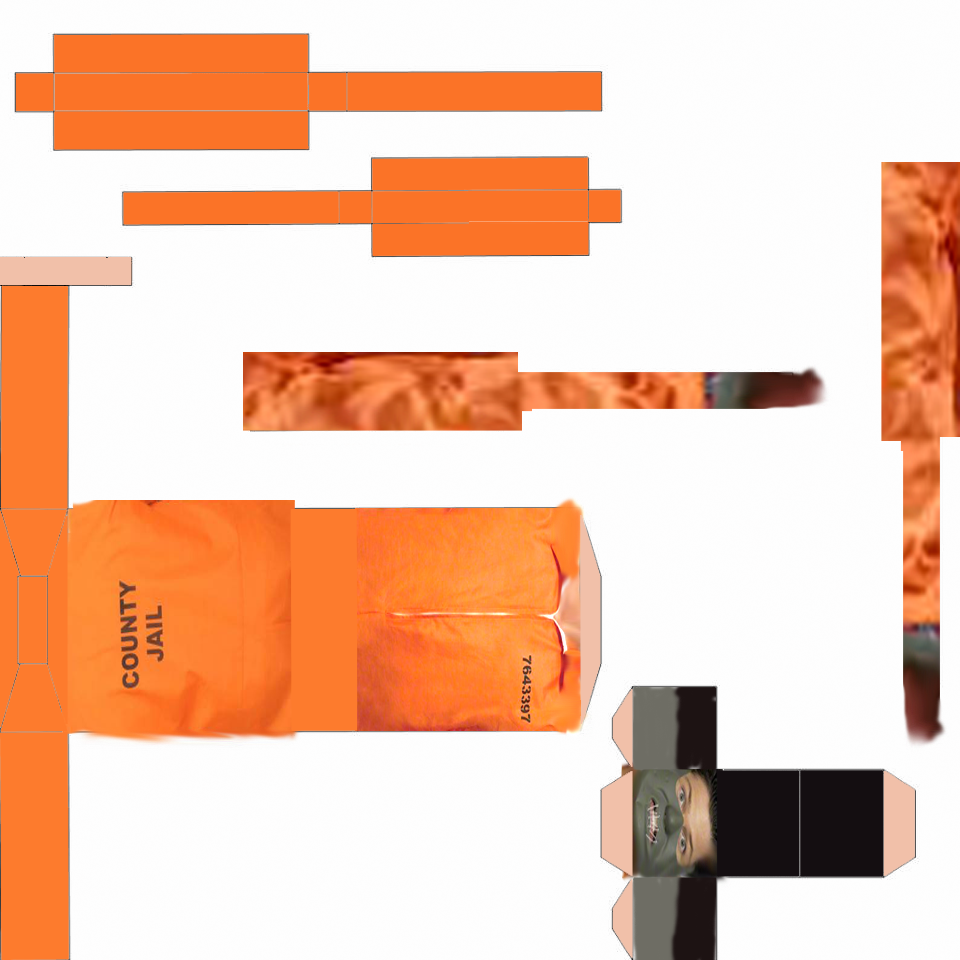
\includegraphics[scale=0.2]{prisonnier.png}
\end{center}
\newpage
Et voici un des ennemis en dehors de la prison : 
\begin{center}
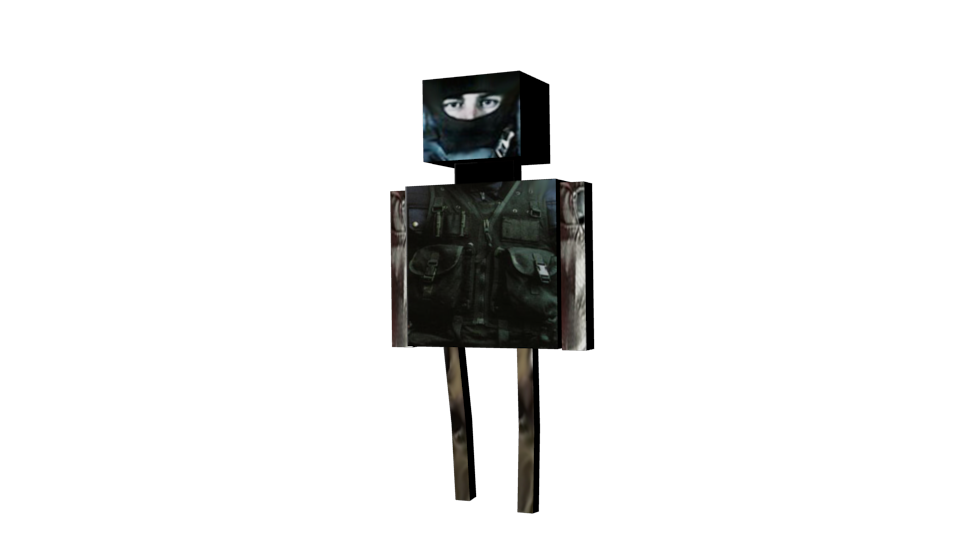
\includegraphics[scale=0.8]{ennemidehorsblend.png}
\end{center}
\begin{center}
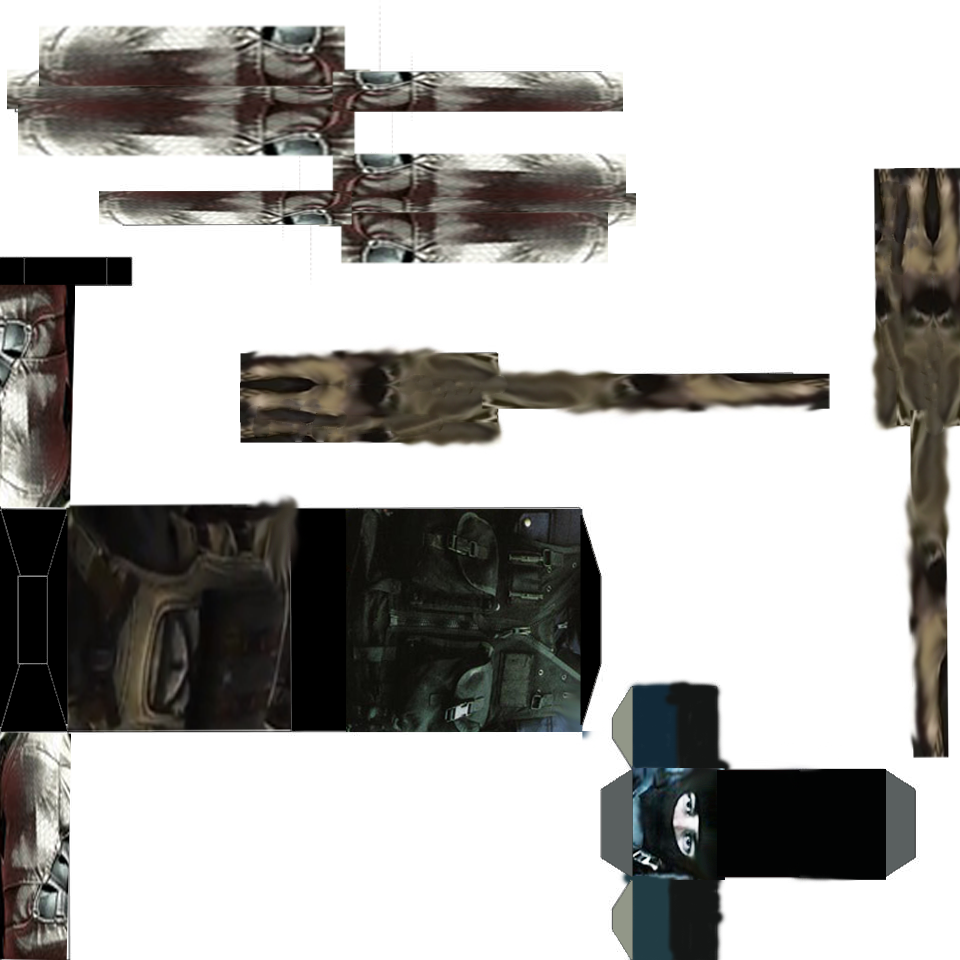
\includegraphics[scale=0.2]{ennemidehors.png}
\end{center}
\par
Cependant dessiner des personnages reste un aspect graphique. J’ai dû en effet toucher au code des classes pour pouvoir les insérer. Avec l’aide de Khalis, qui s’est occupé d’autres personnages, j’ai donc terminé les classes Pnj, Objets Utilitaires et Outils.
De même je m’étais occupe dans la première soutenance des classes Décors, Murs et Objets. Pour parfaitement les terminer j’ai dû effectuer les mêmes étapes que pour les personnages.
\newpage
Voici le modèle des murs :
\begin{center}
\includegraphics[scale=0.5]{mur_patron.png}
\end{center}
Voici une des textures utilises :
\begin{center}
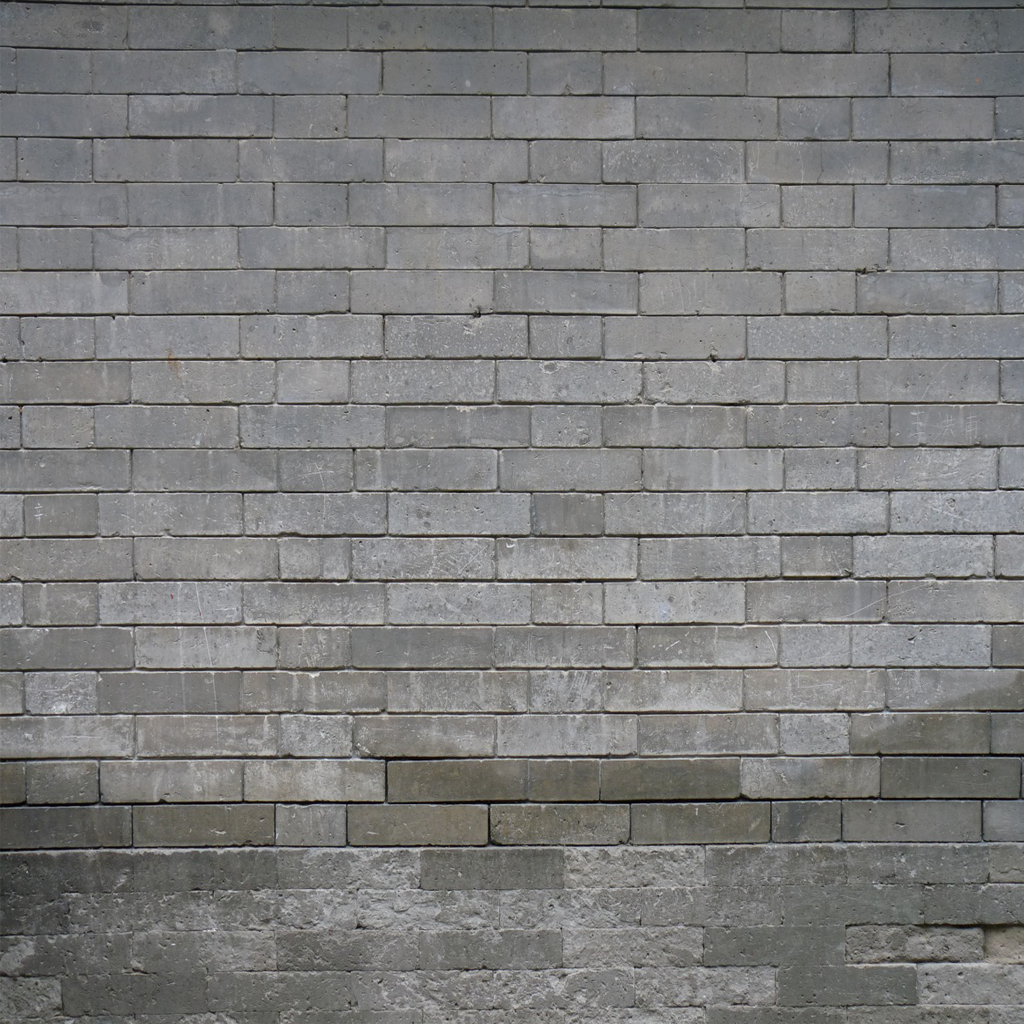
\includegraphics[scale=0.5]{mur_brique.png}
\end{center}
\par
Par ailleurs je me suis aussi occupe du réseau avec XNA mais le sujet etant assez complexe je n'ai pas pu le terminer pour cette soutenance. Je compte m'en occuper lors de la derniere.
\subsubsection{Et après ?}
\par
Pour notre troisième soutenance je vais me fixer quelques objectifs à atteindre :
\newline

\par
\underline{Le multijoueur et le réseau}
\newline
\par
Je compte terminer le multijoueur car même si aujourd'hui il est fonctionnel, je compte l'améliorer.Aussi j'aimerais que les scores des joueurs puissent s'afficher et qu'ils puissent communiquer entres eux. Cela me permettra de progresser dans le code aussi.
\newline

\par
\underline{Les sons}
\newline
\par
Je compte rajouter des sons pour que l'ambiance du jeu soit complète lors de la troisième soutenance avec l’aide d’Anatole.
\newline

\par
\underline{Remerciements}
\newline
\par
Comment ne pas terminer encore une fois sur des remerciements à mon groupe qui reste soudé malgré nos différents? C'est donc pour cela que je remercie notre leader Louis qui soude quotidiennement notre équipe et nous encourage lorsque certains problèmes sont rencontrés, notre visionnaire Anatole qui aide à la projection du projet ainsi qu'à son aboutissement et toujours Khalis qui amène la bonne humeur tous les jours.

\newpage

\subsection {Anatole\textcolor {pseudoblue} {\textit {"Totonut"}} Moreau}
\newpage
\begin{tabular}{|c|p{2cm}|p{2cm}|p{2cm}|}


\hline
& Première soutenance & Deuxième soutenance & Troisième soutenance\\ 
\hline

Codage décors & 70\% & 100\% & 100\%\\
\hline
Codage objets & 70\% & 100\% & 100\%\\
\hline
Codage personnages & 70\% & 90\% & 100\%\\
\hline

Graphismes 2D/3D & - & 60\% & 100\%\\
\hline

Site web & 70\% & 100\% & 100\%\\
\hline

Son & 20\% & 80\% & 100\%\\
\hline

Collisions & - & 50\% & 100\%\\
\hline

Affichage & 70\% & 100\% & 100\%\\
\hline

Boucle de jeu & - & 50\% & 100\%\\
\hline

Interaction entre éléments du jeu & 20\% & 70\% & 100\%\\
\hline

Menu & 50\% & 100\% & 100\%\\
\hline

Réseau & - & 100\% & 100\%\\
\hline

Multijoueur & - & 60\% & 100\%\\
\hline

\end{tabular}

\section{Conclusion}
\par
Pendant notre période de travail, nous avons pris de l’avance sur nos prévisions ce qui nous permet de bien perfectionner certains détails.
\par
En effet, de nombreuses idées furent ajoutées  et les tâches que nous nous étions données à respecter depuis la première soutenance ont été remplies. Nous souhaitons vous montrer les avancées que nous avons réalisées car nous n’en sommes pas peu fiers !
\par
Notre jeu nous satisfait pour le moment mais nous ne nous relâchons pas et nous espérons que la soutenance se déroule dans les meilleures conditions.

\end{document}
